\documentclass[a4paper]{article}

%%%%%%%% CREATE DOCUMENT STRUCTURE %%%%%%%%
%% Language and font encodings
\usepackage[english]{babel}
\usepackage[utf8x]{inputenc}
\usepackage[T1]{fontenc}
%\usepackage{subfig}

%% Sets page size and margins
\usepackage[a4paper,top=3cm,bottom=2cm,left=2cm,right=2cm,marginparwidth=1.75cm]{geometry}

%% Useful packages
\usepackage{amsmath}
\usepackage{graphicx}
\usepackage[colorinlistoftodos]{todonotes}
\usepackage[colorlinks=true, allcolors=blue]{hyperref}
%\usepackage{caption}
\usepackage[justification=centering]{caption}
\usepackage{subcaption}
\usepackage{sectsty}
\usepackage{float}
\usepackage{titling} 
\usepackage{blindtext}
\usepackage[square,sort,comma,numbers]{natbib}
\usepackage[colorinlistoftodos]{todonotes}
\usepackage{xcolor}
\usepackage{fancyhdr}
\usepackage{lipsum}

%% definitions 
\definecolor{darkgreen}{rgb}{0.0, 0.4, 0.0}

%% Define your personal info here %%%%%%%%%%%%%%%%%%%%%%%
\newcommand\TPid{0}
\newcommand\TPname{Stohastic processes}
\newcommand\Firstname{Joao Filipe}
\newcommand\Familyname{Costa da Quinta}
\newcommand\Email{Joao.Costa@etu.unige.ch}

%%%%%%%%%%%%%%%%%%%%%%%%%%%%%%%%%%%%%%%%%%%%%%%%%%%%%%%

%%%%%%% Page header %%%%%%
\pagestyle{fancy}
\fancyhf{}
\rhead{TP \TPid: \TPname}
\lhead{\Firstname \Familyname}
\rfoot{Page \thepage}


%%%%%%%% DOCUMENT %%%%%%%%
\begin{document}

%%%% Title Page
\begin{titlepage}

\newcommand{\HRule}{\rule{\linewidth}{0.5mm}} 							% horizontal line and its thickness

\center 
 
% University
\textsc{\LARGE Université de Genève}\\[1cm]

% Document info
\textsc{\Large Metaheuristics for optimization}\\[0.2cm]									% Course Code
\HRule \\[0.8cm]
{ \huge \bfseries TP \TPid : \TPname}\\[0.7cm]								% Assignment
\HRule \\[2cm]
\large
\emph{Author:} \Firstname \; \Familyname\\[0.5cm]		
\emph{E-mail:} {\color{blue}\Email}\\[7cm]		
% Author info
% Author info
{\large \today}\\[2cm]

\includegraphics[width=0.4\textwidth]{images/unige_csd.png}\\[1cm] 	% University logo
\vfill 
\end{titlepage}


% ============================================
% ----------------------------------
\newpage
\section*{Simulation of a balanced dice}
\subsection*{Intro and methodology}
During this exercise we will be simulating rolls of a N-face balanced dice. This means that the dice has N possible outcomes at each throw, all faces are equally likely with a probability of 1/N.\\
For each roll we need to do the following tasks:
\begin{itemize}
\item [(1)] compute a new random value $r \in [0,1)$, done with random() function from random package
\item [(2)] compute $i = \lfloor N * r \rfloor$, done with floor() function from math package
\end{itemize}
After doing the three tasks, we get a value, that is the simulated roll.\\
The following graphic represents this phenomenon for N = {6, 15}\\
\begin{figure}[H]
\center
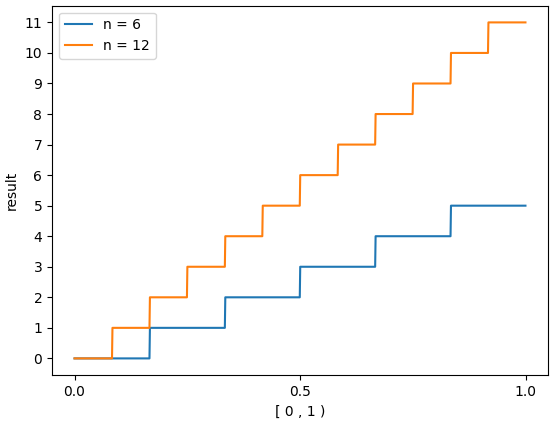
\includegraphics[width=0.4\textwidth]{images/balanced_dice.PNG}
\caption*{Values for N = $\{6, 12\}$}
\end{figure}
In the image above we see this kind of step function, this is due to the fact that we use the function .floor().\\
The function that does this computation can be found in the functions.py file, and its signature is the following:
\begin{center}
balancedDice(N), where N corresponds to the number of faces in the balanced dice.
\end{center}
To check if the function works well we simply use it a large amount of times, or n times, if all faces are represented the same amount of times we know it is a good simulation. Obviously we need n to be large enough.
\subsection*{Results}
For our results we will run the script with N = 6, and n = $\{ 100, 1000, 10000\}$.\\
To 'read' the results, we will be computing the frequency of each face. Let's say the face represented by the value 1 was seen 20 times out of 100 rolls, then its frequency is 20/100 = 0.2.

\begin{table}[H]
\begin{center}
\begin{tabular}{|c|c|c|c|c|c|c|}
\hline
Face                   & 1      & 2     & 3      & 4      & 5      & 6      \\ \hline
100 rolls   & 0.18   & 0.21  & 0.15   & 0.18   & 0.15   & 0.13   \\ \hline
1000 rolls  & 0.184  & 0.17  & 0.148  & 0.165  & 0.167  & 0.166  \\ \hline
10000 rolls & 0.1742 & 0.167 & 0.1671 & 0.1663 & 0.1641 & 0.1613 \\ \hline
\end{tabular}
\caption*{\label{BD} Frequency of each face for different number of rolls}
\end{center}
\end{table}
The perfect frequency is $(n/N)/n = 0.166$ for $N = 6$ and $n = \{100, 1000, 10000\}$. We can easily see that we get closer to the perfect frequency as n becomes larger.\\

% ----------------------------------
\newpage
\section*{Simulation of a biased dice as a balanced dice}
\subsection*{Intro and methodology}
A biased dice is a N-face dice, where all faces are equally likely. Which means we can't use the same function as we did in the previous exercise.\\
The solution is to transform the N-face biased dice into a N'-face balanced dice. However, this can only be done if the probabilities are commensurable.\\
To do this we have to:
\begin{itemize}
\item [(1)] find the smallest probability of the biased dice $\longrightarrow p_{min}$
\item [(2)] divide the segment $[0, 1)$ into $1/p_{min} = N'$ divisions, which means that we now have a N'-face balanced dice
\item [(3)] assign the different faces of the N'-face dice to the previous N-face biased dice
\end{itemize}
\begin{table}[H]
\begin{center}
\begin{tabular}{|c|c|c|c|c|c|c|c|c|c|c|c|c|c|c|c|c|}
\hline
\textbf{N-face biased dice}    & \multicolumn{4}{c|}{1} & \multicolumn{4}{c|}{2} & \multicolumn{4}{c|}{3} & \multicolumn{2}{c|}{4} & 5  & 6  \\ \hline
\textbf{N'-face balanced dice} & 1    & 2   & 3   & 4   & 5    & 6   & 7   & 8   & 9   & 10   & 11  & 12  & 13         & 14        & 15 & 16 \\ \hline
\end{tabular}
\caption*{\label{BD} Assignment of N'-face balanced dice to N-face biased dice}
\end{center}
\end{table}
With this table it becomes easy to the exercise. After computing the N'-face balanced dice, we simply use the function from the previous exercise.
\subsection*{Results}
For our results we will run the script with 6-face biased dice of probability P = $[ 1/4, 1/4, 1/4, 1/8, 1/16, 1/16]$. $1/16$ is the smallest probability, which means our balanced dice has 16 faces of $1/16$ probability each. We will do n = $\{ 100, 1000, 10000\}$ number of rolls.\\
To 'read' the results, we will be computing the frequency of each face. Let's say the face represented by the value 1 was seen 20 times out of 100 rolls, then its frequency is 20/100 = 0.2.

\begin{table}[H]
\begin{center}
\begin{tabular}{|c|c|c|c|c|c|c|}
\hline
Face        & 1      & 2      & 3      & 4      & 5      & 6      \\ \hline
100 rolls   & 0.25   & 0.25   & 0.2    & 0.17   & 0.08   & 0.05   \\ \hline
1000 rolls  & 0.253  & 0.234  & 0.258  & 0.137  & 0.052  & 0.066  \\ \hline
10000 rolls & 0.2541 & 0.2511 & 0.2417 & 0.1209 & 0.0657 & 0.0665 \\ \hline
\end{tabular}
\caption*{\label{BD} Frequency of each face for different number of rolls}
\vspace{0.6cm}
\begin{tabular}{|c|c|c|c|c|c|c|}
\hline
Face              & 1    & 2    & 3    & 4     & 5      & 6      \\ \hline
Perfect Frequency & 0.25 & 0.25 & 0.25 & 0.125 & 0.0625 & 0.0625 \\ \hline
\end{tabular}
\caption*{\label{BD} Perfect frequency for each face}
\end{center}
\end{table}
The perfect frequency is different for each face, since they have different probabilities. We can easily see that we get closer to the perfect frequency as n becomes larger.\\


% ----------------------------------
\newpage
\section*{Simulation of a biased coin toss}
\subsection*{Intro and methodology}
A coin toss has 2 possible outcomes, tail with probability p, and head with probability 1-p. For the coin to be balanced, p needs to be 0.5, any other value and the coin is biased.\\
For each coin toss we need to do the following tasks:
\begin{itemize}
\item [(1)] compute a new random value $r \in [0,1)$, done with random() function from random package
\item [(2)] compute $\lambda = \lfloor p + r \rfloor$, done with floor() function from math package
\end{itemize}
$\lambda$ has two possible outcomes $\{0, 1\}$ 0 occurs when $p + r < 1$ and 1 occurs when $1 \leq p + r$. Other values are never possible, as $r < 1$ and $0 \leq p \leq 1$, which means $p + r < 2$ for every p and r.\\
If $\lambda = 0$ then the coin toss resulted in head, if $\lambda = 1$ then the coin toss resulted in tail.
\subsection*{Results}
For our results we will run the script with p = 0.3 biased probability. We will do n = $\{ 100, 1000, 10000\}$ number of tosses.\\
To 'read' the results, we will be computing the frequency of each face. Let's say the face represented by the value 1 was seen 20 times out of 100 rolls, then its frequency is 20/100 = 0.2. The perfect frequency for tail corresponds to p = 0.3, and the perfect frequency to head corresponds to 1 - p = 0.7.

\begin{table}[H]
\begin{center}
\begin{tabular}{|c|c|c|}
\hline
Face         & Tail   & Head   \\ \hline
100 tosses   & 0.39   & 0.61   \\ \hline
1000 tosses  & 0.306  & 0.694  \\ \hline
10000 tosses & 0.3028 & 0.6972 \\ \hline
\end{tabular}
\caption*{\label{BD} Frequency of tail / head for p = 0.3}
\end{center}
\end{table}
Just like in the previous exercises, a larger number of tosses/rolls, results in better results.


% ----------------------------------
\newpage
\section*{Simulation of a biased dice using a biased coin}
\subsection*{Intro and methodology}
In this exercise we will simulate a N-face biased dice. However, this time we will do it by using the coin toss function from exercise 3. Let P = $[ 1/4, 1/4, 1/4, 1/8, 1/16, 1/16]$. $1/16$ be the probability of the 6-face biased dice we want to simulate, to do this we need to:\\
\begin{itemize}
\item [(1)] toss a coin with probability $p = P_{0} = 1/4$ 
\item [(2)] if the result is tail, then the toss was a success, and the the result of the dice throw is 1
\item [(3)] if the result is head, then we need to remove 1/4 of our probability mass, and normalize the probabilities we have left
\item [(4)] toss a coin again, now with the new normalized probability for $p = P_{1}$
\item [(5)] if the result is tail, then we return 2, if it is head, we do point (3) again.
\end{itemize}
\begin{table}[H]
\resizebox{\textwidth}{40px}{
\begin{tabular}{|c|c|c|c|c|c|c|}
\hline
Face        & 1                                    & 2                                    & 3                                    & 4                                    & 5                                    & 6                 \\ \hline
Probability & 1/4                                  & 1/4                                  & 1/4                                  & 1/8                                  & 1/16                                 & 1/16              \\ \hline
toss n.1    & {\color[HTML]{FE0000} \textbf{FAIL}} & (1/4)/(3/4)=1/3                      & (1/4)/(3/4)=1/3                      & (1/8)/(3/4)=1/6                      & (1/16)/(3/4)=1/12                    & (1/16)/(3/4)=1/12 \\ \hline
toss n.2    &                                      & {\color[HTML]{FE0000} \textbf{FAIL}} & (1/3)/(2/3)=1/2                      & (1/6)/(2/3)=1/4                      & (1/12)/(2/3)=1/8                     & (1/12)/(2/3)=1/8  \\ \hline
toss n.3    &                                      &                                      & {\color[HTML]{FE0000} \textbf{FAIL}} & (1/4)/(1/2)=1/2                      & (1/8)/(1/2)=1/4                      & (1/8)/(1/2)=1/4   \\ \hline
toss n.4    &                                      &                                      &                                      & {\color[HTML]{FE0000} \textbf{FAIL}} & (1/4)/(1/2)=1/2                      & (1/4)/(1/2)=1/2   \\ \hline
toss n.5    &                                      &                                      &                                      &                                      & {\color[HTML]{FE0000} \textbf{FAIL}} & (1/2)/(1/2)=1     \\ \hline
\end{tabular}}
\caption*{\label{BD} Normalization example of a 6-face biased dice of probability P = $[ 1/4, 1/4, 1/4, 1/8, 1/16, 1/16]$}
\end{table}

The normalization process is done in the following steps:
\begin{itemize}
\item [(1)] remove the failed toss from the probability mass, for example, if the first throw fails , we have $1 - 1/4 = 3/4$
\item [(2)] compute a new $P\_new$ such that : $P\_new_{i} = P_{i} / (3/4)$
\end{itemize}


\subsection*{Results}
For our results we will run the script with 6-face biased dice of probability P = $[ 1/4, 1/4, 1/4, 1/8, 1/16, 1/16]$. We will do n = $\{ 100, 1000, 10000\}$ number of rolls.\\
To 'read' the results, we will be computing the frequency of each face. Let's say the face represented by the value 1 was seen 20 times out of 100 rolls, then its frequency is 20/100 = 0.2.

\begin{table}[H]
\begin{center}
\begin{tabular}{|c|c|c|c|c|c|c|}
\hline
Face        & 1      & 2      & 3      & 4      & 5      & 6      \\ \hline
100 rolls   & 0.33   & 0.22   & 0.19    & 0.1   & 0.08   & 0.08   \\ \hline
1000 rolls  & 0.245  & 0.259  & 0.261  & 0.12  & 0.057  & 0.058  \\ \hline
10000 rolls & 0.25 & 0.2547 & 0.245 & 0.1249 & 0.0633 & 0.0621 \\ \hline
\end{tabular}
\caption*{\label{BD} Frequency of each face for different number of rolls}
\vspace{0.6cm}
\begin{tabular}{|c|c|c|c|c|c|c|}
\hline
Face              & 1    & 2    & 3    & 4     & 5      & 6      \\ \hline
Perfect Frequency & 0.25 & 0.25 & 0.25 & 0.125 & 0.0625 & 0.0625 \\ \hline
\end{tabular}
\caption*{\label{BD} Perfect frequency for each face}
\end{center}
\end{table}
The perfect frequency is different for each face, since they have different probabilities. We can easily see that we get closer to the perfect frequency as n becomes larger.\\

% ----------------------------------
\newpage
\section*{Simulation of the Roulette method}
\subsection*{Intro and methodology}
This is yet another method in which we can simulate a N-face biased dice.\\
This method is very easy to understand, let's see what the steps are:
\begin{itemize}
\item [(1)] from probability P, compute $P\_comul$ where $P\_comul_{i}$ is equal to the sum of every probability $P_{j}$ such that $0 \leq j \leq i$
\item [(2)] compute a new random value $r \in [0,1)$, done with random() function from random package
\item [(3)] check which $P\_comul_{i} < r$, starting from i = 0, the first $P\_comul_{i}$ that respects this condition, is the i we return
\end{itemize}

\begin{table}[H]
\begin{center}
\begin{tabular}{|c|c|c|c|c|c|c|}
\hline
$P$        & 1/4 & 1/4 & 1/4 & 1/8   & 1/16      & 1/16      \\ \hline
$P\_comul$ & 1/4 & 2/4 & 3/4 & 7/8 & 15/16 & 16/16 = 1 \\ \hline
\end{tabular}
\caption*{\label{BD} Computation of $P\_comul$ for P = $[ 1/4, 1/4, 1/4, 1/8, 1/16, 1/16]$ }
\end{center}
\end{table}
\end{document}
